\section{Soft constraint automata : 2 pages}

\paragraph{Constraints}
Consider a fixed rational component. The relation between its ports is realized by constraints. In addition to the previously defined set P of ports variables $v\in P$, we define the countably infinite set $M$ of memory cells, disjoint with $P$. Memory cells can be intuitively understood as variable storage for components. Let $m \in M$, then by $\underline{m}\in \underline{M}$ we denote the variable for current value, and by $\underline{m}'\in \underline{M}'$ we denote the variable for the next value. The constant symbol $*$ represents no activity. The symbol $f$ [resp. $R$] stands for a function [resp. relation] with fixed arity $n$. 

\begin{definition} A \textbf{term} is defined inductively as:
	$$ t ::= \quad v \quad | \quad \underline{m} \quad | \quad \underline{m}' \quad | \quad f(t_1, ..., t_n) \quad | \quad * $$
	A \textbf{constraint} is a formula $\phi$ defined inductively by:
	$$ \phi ::= \quad \bot \quad |\quad t_1 = t_2 \quad|\quad R(t_1, ... , t_n) \quad|\quad \phi_1 \land \phi_2 \quad| \quad \neg \phi \quad| \quad \exists x \phi $$
\end{definition}

We use $\neg (t_1=t_2) := t_1 \not = t_2$ and $\phi_1 \lor \phi_2 := \neg (\neg \phi_1 \land \phi_2)$. Let $V_{\phi}$ refers to the set of free variables in $\phi$.
\paragraph{Model} 
Terms are interpreted as data values from the set of $D$ data. We define $\gamma:P\cup \underline{M'} \cup \underline{M} \rightarrow D$ the assignment map for variables and memory cells. We note $t^D$ the interpretation of the term $t$ in the data domain $D$. Thus, $v^D=\gamma(v)$, $\underline{m}^D=\gamma(\underline{m})$ and $\underline{m}'^D=\gamma(\underline{m}')$. Functions $f$ of arity $n$ are interpreted as $f^{D}:D^n \rightarrow D$ and $*^D\in D$ as the data symbol $*$. Relation $R$ of arity $n$ are interpreted as $R^D : D^n \rightarrow 2$. \begin{definition}
	Given a constraint $\phi$, we inductively define the \textbf{satisfaction} relation $D, \gamma \models \phi$ with :
\begin{align*}
	 D, \gamma \not\models \bot   \quad &; \quad \quad D, \gamma \models t_1=t_2 \quad \Leftrightarrow \quad t_1^D=t_2^D; \\
	 D, \gamma \models \phi_1=\phi_2 \quad &\Leftrightarrow \quad D, \gamma \models \phi_1\text{ and }D, \gamma \models \phi_2 ; \\
	 D, \gamma \models R(t_1,...t_n) \quad &\Leftrightarrow \quad (t_1^D,...t_n^D) \in R^D; \\
	 D, \gamma \models \exists x\phi \quad &\Leftrightarrow \quad D, \gamma[x \mapsto m ] \models \phi \text{ for some m} \in D.
\end{align*}	
\end{definition}
We refer to the basic intuition of the reader to define the assignment update $\gamma[x \mapsto m]$.
\paragraph{Solving} 
The solutions of a constraint $\phi$ is the set of all assignment maps such that the constraint is satisfied, $i.e.$ $\Gamma_{\phi} = \{ \gamma \mid D,\gamma \models \phi \}$. 
%We call $\Gamma_C:V_C \rightarrow D\cup\{\varnothing\}$ the assignment map defined on the set of variable $V_C$ of a component $C$. Given $v\in V_C$, $\Gamma_C(v) = d \in D$ if $v$ is defined, or $\Gamma_C(v) = \varnothing$ if v is not defined. We consider initially a map $\Gamma_C$ on which some variables already have a value assigned ($\Gamma_C(v) \not = \varnothing$).

%We say that a port $p$ fires whenever $p \not = *$. If a port $p$ fires and the port equates another port $q$, then both ports must synchronize and observe the same data. The corresponding formula is : $p=q \land p \not= *$. The symbol $*$ models the case where no data is observed at the port or in the memory cell. Existential quantifier is equivalent to hiding a port. Once hidden, it is no longer possible to synchronize on the port, and the variable can be eliminated by substitution. We allow user defined functions and relation in our language. Since a variable can be shared with the environment, we call $pending$ value the value set by the environment on a free variable.

%We say that a constraint is satisfiable if there is an assignment for all its free variables that makes the constraint true. Finding such an assignment follows two steps. Lets call $\Gamma:V \rightarrow D\cup\{*\}$ the assignment map from variable to data or special symbol *. For each constraints, we start with an assignment map $\Gamma$ empty, meaning that all variables maps to $*$. We first look at all free variables involved in the constraint and update the map $\Gamma$ according to their $pending$ value.

\paragraph{Preferences} 
In practice, an implementation would have to choose non deterministically an assignment from the set. We want to define such a partial order among assignments. We introduce c-semiring, an algebraic structure that induces a partial order.

%Intuitively, constraints serve as guards for transition in SCA. From one state, if multiple constraint are satisfiable, multiple transitions could be taken. Since we want to locally determine which transition to take, we introduce csemiring, an algebraic structure that induces an order on the transitions.

\begin{definition} A \textbf{c-semiring} is a non-empty set $(E, +, \times, \boldmath{1},\boldmath{0} )$, such that:
	\begin{list}{-}{ }
		\item $(E,+)$ is an idempotent commutative monoid \\ 
			\text{ \quad \quad \quad \quad \quad} with identity element 0 and absorbing element 1. 
		\item $(E,\times)$ is a commutative monoid \\
			\text{ \quad \quad \quad \quad \quad} with identity element 1 and absorbing element 0.
		\item Multiplication distributes over addition from either sides.
	\end{list} 
\end{definition}
Let $A \subset E$, we use the prefix notation $\sum(A)$ to describe the sum of all elements of A.
A csemiring admits a partial order $\leq_{E}$, defined as the smallest relation satisfying:
$$ \frac{e,e' \in E \quad e+e' = e'}{e \leq_{E} e'} $$
Given two constraints $\phi_1,\phi_2 \in C$ and elements $e_1,e_2 \in E$, we call soft constraint the tuples $(\phi_1,e_1)$, $(\phi_2,e_2)$. We say that $(\phi_1,e_1)\leq(\phi_2,e_2)$ if and only if $e_1 \leq_E e_2$, $i.e.$ $\leq_E$ lifts to a partial order among soft constraints. 

Since the order is partial, the element of the c-semiring need not always be comparable. 
Given a set of constraints $C$ and a c-semiring $E$, the induced set of soft constraint is $C\times E$. For a soft constraint $(\phi,e) \in C \times E$, we note $\Gamma_{\phi,e} = \{ (\gamma,e) \mid D,\gamma \models \phi \}$ the set of solutions.

\begin{definition}
	\textbf{Soft constraint automata} (sca) is a tuple $(Q, \rightarrow, C \times E, q_{0} )$ where: 
	\begin{list}{-}{ }
		\item $Q$ is a set of states and $q_0\in$ Q is the initial state.
		\item C $\times E$ is a set of soft constraints.
		\item $\rightarrow \subseteq Q \times C \times E \times Q$ is a finite relation called transition relation. 
		%A transition is denoted by $\left\langle q_i, c, s, p_i \right\rangle \in \rightarrow$
	\end{list}
\end{definition}
For clarity, we identify the tuple $(q,\phi,e,q') \in \rightarrow$ with the notation $q \xrightarrow{\phi,e} q'$.
\paragraph{Operational semantic}
Let $A = (Q, \rightarrow, C \times E, q_{0} )$ be a soft constraint automaton. Given $q\in Q$, we note:
% $$C(q) = \biguplus_{q' \in Q}\{(c,e) \mid q \xrightarrow{(c,e)}q' \}$$
 $$̀\Gamma(q) = \biguplus_{(q,\phi,e,q') \in \rightarrow}\Gamma_{\phi,e} $$
$\Gamma(q)$ corresponds to the disjoint sum of solutions for soft constraints present on an outgoing transition of state $q$. Being in the context of an open system, the value of a port can be influenced by the environment. We call $\Delta \subseteq \Gamma(q) $ the restriction made by the environment on possible set of assignment. We remark that the map $\gamma_*$ defined as $ \gamma_*(x) = 
\begin{cases}
	* &\quad\text{if x}\in P \\ 
	\underline{x} &\quad\text{if x} \in M  
\end{cases}$
 is always contained in $\Delta$. If $|\Delta|=1$, $\gamma_*$ is the only possible assignment. If $\Delta = \Gamma(q)$, the environment does not remove any possible assignment. Assuming a $\Delta \subseteq \Gamma(q)$ from the environment, we define the set of $best$ assignment as $$\bigwedge\Delta= \{(\gamma, e) \mid e' \leq_E e \textit{ for all } (\gamma',e')\in \Delta \}$$ Since the sum $\Gamma_q$ is disjoint, we can define $p : \bigwedge\Delta \rightarrow Q$, a function that choose non deterministically a tuple from $\bigwedge\Delta$, and return the next state in $A$.
%We call $\Delta_{\psi} = \{ \delta \mid D,\delta \models \psi \}$ the partial map that models the environment assignment. Since the environment is represented by an irrational component, it is not possible to finitely represents the relation on its ports as a constraint. However, we know that $V_{\psi} \cap V_{\phi} \not = \emptyset$ since $\phi$ has some free variables. Thus, in each state we take 

%We define the semantic of soft constraint automata $\mathcal{A} = \left\langle Q, \rightarrow, C, \mathbb{S}, q_{0} \right\rangle$ as follows.
%At each state $q$, we take the set of constraint $\mathcal{C}_q = \{c \in C | \exists q'\in Q, q \xrightarrow{(c,e)} q' \in \mathcal{A}\}$. For each constraint $c\in \mathcal{C}_q$, 
%Given a sca $A = \left\langle Q, \rightarrow, C, \mathbb{S}, q_{0}, \right\rangle$, and a state $q\in Q$, the operational semantic of Soft Constraint Automata follows two steps : assignment and constraint solving. We denote $V_c$ the set of free variables involved in the constraint $c \in C$ The assignment step takes all variables involved in the constraints and assign values defined by the environment. Since variables refer to ports or current (or next value of memory cells), assigning a value means reading the value from a port. Since a port can have no data (*) or the variable no value assign, the second step invoke a constraint solver to find an assignment to satisfy the constraint.

%\paragraph*{LTS}

\begin{example}
	We present the example of a dancing flying drone, and we show the description of a non trivial behavior. The component has four ports: $p_{west}$, $p_{east}$, $p_{north}$ and $p_{south}$. Each port is constrained by a formula. We note $east$, $west$, $south$ and $north$ the name of the constraint respectively responsible to the observable behavior moving east, west, south or north. Certain actions are mutually exclusives : it is not possible to move east and west, or south and north at the same time. This composability relation appears in the formulation of the constraint. We define : 
	\begin{align*}
		& \text{west} := p_{west} \not = * \land p_{east} = * \\
		& \text{east} := p_{east} \not = * \land p_{west} = * \\
		& \text{north} := p_{north} \not = * \land p_{north} = * \\
		& \text{south} := p_{south} \not = * \land p_{south} = * 
	\end{align*}

	\begin{figure}[t]
	\centering
	\label{fig:Components}{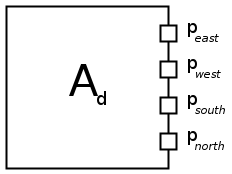
\includegraphics[scale=0.4]{pic/dancing_drone.png}}
	\qquad
	\caption{Soft constraint automata $A_d$ modeling the dance of the drone}
	\end{figure}
	
	\begin{figure}[H]
		\centering
		\resizebox{8cm}{!}{ \begin{tikzpicture}[>=latex,shorten >=1pt,node distance=3cm,on grid,auto, node/.style={circle,draw,minimum size=25pt}, ]

 \node[state] (qW) at (-40pt,0pt) {$q_W$};
 \node[state, right = of qW] (qN) {$q_N$};
 \node[state, below = of qW] (qS) {$q_S$};
 \node[state, right = of qS] (qE) {$q_E$};
 \draw[<-,text=white] (qW) -- node[] {} ++(0,1);
 \draw[->] (qN) to[out=160,in=20] node[above] {west , 2} (qW);
 \draw[->] (qS) to[out=-20,in=200] node[below] {east , 2} (qE);
 \draw[->] (qW) to[out=-110,in=110] node[left] {south , 2} (qS);
 \draw[->] (qE) to[out= 80,in=-80] node[right] {north, 2} (qN);
 \draw[->] (qN) to[out=20,in=-20,looseness=8] node[right, align=left] {east , 3\\south , 3 \\ north, 3} (qN);
 \draw[->] (qE) to[out=20,in=-20,looseness=8] node[right, align=left] {east , 3\\south , 3 \\ west, 3} (qE);
 \draw[->] (qW) to[out=160,in=-160,looseness=8] node[left, align=left] {west , 
 3 \\ east, 3 \\ north, 3} (qW);
 \draw[->] (qS) to[out=160,in=-160,looseness=8] node[left, align=left] {west , 3\\ south , 3 \\ north, 3} (qS);
 \end{tikzpicture}}
		\caption{Soft constraint automata $A_d$ modeling the dance of the drone}
		\label{moveSCA}
	\end{figure}

	The possible behaviors generated by the soft constraint automata of Fig. 2 correspond to the set of stream $\Sigma^{\omega}$, where a stream $\sigma \in \Sigma^{\omega}$ represents a trace of successive actions. The stream $(west,3)^{\omega} \in \Sigma^{\omega}$ represents the trace where the dancing drone always took the action $west$ in the initial state. As shown previously, the c-semiring value associated to the constraint induces a partial order on the set of behavior. In this example, if all constraints could be satisfied in each states, the best transition is the transition involving the soft constraint with the preference $2$. Thus, the best behavior is the stream $((south,2),(east,2),(north,2),(west,2))^{\omega}$, which corresponds to the dancing square of the drone.
	%$\{(west,3)^{\omega}, (east,3)^{\omega}, ((east,3),(south,2),(east,3)^{\omega}), ...\}$

%	This example present a protocol between three components : $east$,$west$ and $stay_{lon}$. Each components have one port, respectively named $p_{east}$, $p_west$ and $p_{stay_{lon}}$; and define a constraint $east := p_{east} \not = *$, $west := p_{west} \not = *$ and $stay_{lon} := p_{stay_{lon}} \not = *$. The constraint $idle := \neg east \land \neg west \land \neg stay_{lon}$ represents the assignment $\gamma_*$. We use the weighted c-semiring $(\mathbb{R}_+,+,\min,+\infty,0)$ and construct the following soft constraint automaton:
%	\begin{figure}[H]
%		\centering
%		\resizebox{8cm}{!}{ \begin{tikzpicture}[>=latex,shorten >=1pt,node distance=3cm,on grid,auto, node/.style={circle,draw,minimum size=25pt}, ]

 \node[state] (q0) at (-40pt,0pt) {$q_W$};
 \node[state, right = of q0] (q1) {$q_E$};
 \draw[<-,text=white] (q0) -- node[] {} ++(0,1);
 \draw[->] (q1) to[out=200,in=-20] node[below] {west , 5} (q0);
 \draw[->] (q0) to[out=20,in=160] node[above] {east , 5} (q1);
 \draw[->] (q1) to[out=20,in=-20,looseness=8] node[right, align=left] {east , 0\\stay$_{lon}$ , 5} (q1);
 \draw[->] (q0) to[out=160,in=-160,looseness=8] node[left, align=left] {west , 0\\ stay$_{lon}$ , 5} (q0);
 \end{tikzpicture}
}
%		\caption{Soft constraint automata for moving}
%		\label{moveSCA}
%	\end{figure}
\end{example}
\vfill